\chapter{Statistische Mechanik und Thermodynamik}

    \section{Fragestellung}

\begin{center}
    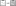
\includegraphics[width=0.6\textwidth]{Abb/1_1.pdf}
\end{center}
Obwohl durch mikroskopische Theorien, wie der Quantenmechanik, die Beschreibung
von Systeme exakt gelingt, ist diese Methode nur für wenige Teilchen sinnvoll.
Einen praxistauglichen Ansatz liefert die statistische Mechanik. Hierbei wird
von einer mikroskopischen Beschreibung, links im Bild dargestellt durch einzelne
Teilchen im Topf, zu einer Makroskopischen, rechts durch große Untersysteme, die
selbst einige Millionen Teilchen beinhalten, übergegangen. Der Schritt hin zu
makroskopischen Messgrößen, die diese Untersysteme charakterisieren, soll nun
die erste Unternehmung sein.

    \subsection{Viele mikroskopische Freiheitsgrade - Mikrozustände}

klassische Mechanik: $\{\vv{r}_i, \vv{p}_i\} \quad i = 1, \dots , N$\\
$\rightarrow$ 6N Freiheitsgrade

\begin{align*}
    &\dot{\vv{r}_j} = \frac{\partial H}{\partial \vv{p}_j} \left( \{
                      \vv{r}_i, \vv{p}_i \} \right) \quad j = 1, \dots, N\\
    &\dot{\vv{p}_j} = - \frac{\partial H}{\partial \vv{r}_j} \left( \{
                         \vv{r}_i, \vv{p}_i\}\right)
\end{align*}

\paragraph{Beispiel:} freies Gas hat 6N-Freiheitsgrade\\
    \indent Quantenmechanik: $\Psi \left( \vec{r}_1, \dots, \vec{r}_n \right)$\\
    \[
        i \hbar \partial_t \Psi \left( \vec{r}_1, \dots, \vec{r}_n \right) =
        \hat{H} \Psi \left( \vec{r}_1, \dots, \vec{r}_n \right)
    \]

\paragraph{Bemerkung:} Ein Mikrozustand ist durch $\Psi$ nur auf einen
Eichfreiheitsgrad bestimmt.

\paragraph{Mikrozustand:} Ein Mikrozustand wird durch die Angabe aller Werte
festgelegt, welche die angenommenen Freiheitsgrade einnehmen. In der klassischen
Mechanik durch einen Vektor, der Orts- und Impulskoordinaten aller Teilchen
enthält. In der Quantenechanik durch eine Vielteilchenwellenfunktion.

\paragraph{Beobachtung:} Physikalische Observable sind oft Beschreibungen von
Systemen und Phänomenen, die sehr viele Teilchen umfassen: $ N \approx 10^{23} $.
So viele Teilchen/Freiheitsgrade kann man in den mikroskopischen Theorien in der
Praxis nicht handhaben. Das will man aber auch gar nicht!

    \subsection{Beobachtungsgrößen - Makrozustände}

Bei einer makroskopischen Betrachtung unserer Systeme, gibt es einige wichtige
Größen:\\
\begin{tabular}{l l l}
N &Teilchenzahl &($\Delta N$)\\
V &Volumen      &($\Delta V$)\\
T &Temperatur   &($\Delta T$)\\
p &Druck        &($\Delta p$)\\
E &Energie      &($\Delta E$)
\end{tabular}\\

\noindent
Beobachtet werden:
\begin{itemize}
    \item Druck-Temperatur-Kurve
    \item Energiedichten
\end{itemize}

weitere Größen: Magnetisierung, supraleitende Energielücke, Phasendiagramme, etc.

\paragraph{Makrozustand:} Der Makrozustand wird durch die Angabe eines vollständigen
Satzes makroskopischer Beobachtungsgrößen definiert. Die Aufgabe der statistischen
Physik ist es, die Dynamik/das Verhalten der makroskopischen Observablen aus den
mikroskopischen Gesetzen heraus zu verstehen und womöglich herzuleiten.

    \section{Statistische Theoriebildung}
    \subsection{Das Versagen des idealtypischen Vorgehens}

